% architecture overview

\chapter{Overview of \CTOS{} Framework}
\label{chap:overview}

The ultimate goal of research on certified OS kernels is not just
to verify the functional correctness of a particular kernel, but
rather to find the best OS design and development methodologies that
can be used to build provably reliable, secure, and efficient computer
systems in a cost-effective way. I enumerate a few important
dimensions of concerns and evaluation metrics which we have used so far
to guide our work toward realizing this goal:
%%%%%%%%%
\begin{itemize}
\item {\bf Support for new kernel design.}  Traditional OS kernels use
  the hardware-enforced ``red line'' to define a single system call
  API. A certified OS kernel opens up the design space significantly as
  it can support multiple certified kernel APIs at different
  abstraction levels. It is important to support kernel
  extensions~\cite{bershad95,engler95} and ring-0
  processes~\cite{hunt07} so we can experiment and find the best trade-offs.
%%%%%%%%%  
\item {\bf Kernel performance.} Verification should not
  impose significant overhead on kernel performance. Of course,
  different kernel designs may imply different performance
  priorities.  An L4-like microkernel~\cite{liedtke95} would sacrifice
  portability for faster inter-process communication (IPC) while a
  Singularity-like kernel~\cite{hunt07} would focus on efficient
  support for type-safe ring-0 processes.
%%%%%%%%%
\item {\bf Verification of global properties.}
  A certified kernel is much less interesting if it cannot be
  used to prove global properties of the complete system built on top
  of the kernel.  Such global
  properties include not only safety, liveness, and security properties
  of user-level processes and virtual machines, but also resource usage
  and availability properties (\eg, to counter denial-of-service attacks).
%%%%%%%%%  
\item {\bf Quality of kernel specification.}  A good kernel
  specification should capture precisely those {\em contextually observable}
  behaviors in the kernel implementation~\cite{dscal15}. It must
  support transferring global properties proved at a high abstraction
  level down to any lower abstraction level.
%%%%%%%%%
\item {\bf Cost of development and maintenance.} Compositionality
  is the key to minimize such cost. If the machine model is stable,
  verification of each kernel module should only need
  to be done once (to show that it {\em implements} its deep
  functional specification~\cite{dscal15}). Global properties should
  be derived from the kernel specification alone. 
%%%%%%%%%  
\item {\bf Quality of formal proofs.} We use the term {\em certified
  kernels} rather than {\em verified kernels} to emphasize
  the importance of third-party machine-checkable proof
  certificates~\cite{shao10}. Hand-written paper proofs are
  error-prone~\cite{findler12}. Program verification without
  machine-checkable proofs has been subject to significant
  controversy~\cite{demillo77}.
\end{itemize}
%%%%%%%%%


Our new \CTOS\ architecture aims to address all of the above concerns
and also tackle all four challenges described in Chapter~\ref{chap-intro}.
The \CTOS\ architecture 
proposes a new language-based account of 
\emph{certified abstraction layer}
to construct certified OS kernels with respect to \emph{deep specifications}.

A {\em certified abstraction layer} is a language-based account that
consists of a triple $\layer{L}{M}{L'}$ plus a mechanized proof
object for the predicate $\ltyp{L}{R}{M}{L'}$,
showing that the layer implementation $M$, built on top of the
interface $L$ (the {\em underlay}), is a {\em contextual refinement}
of the desirable interface $L'$ above (the {\em overlay}). 
We call $L'$ 
a 
\emph{deep
specification} of the module $M$, because it captures
everything {\em contextually observable} about running the module over
its underlay  $L$. Once the certified abstraction layer
is built for module  $M$, there is no need to ever look at $M$
again, and any property about the observable behavior of $M$ can be proved using $L'$ alone. Of
course, if the semantics of the underlying abstract machine (for $M$)
changes, the deep specification for $M$ may also have to change.

Abstraction layers and deep specifications
are our key technologies to address all the challenges 
for constructing certified OS kernels.
Thus, the first question to answer in this thesis
is \emph{why they  work so well for OS kernel verification?}


\section{Why Abstraction Layers?}
\label{sec:overview:why}
To answer the question,
we first describe the main ideas behind deep
specifications and then show why they work more naturally with
abstraction layers than with regular software modules.

\paragraph{Shallow vs. deep specifications}
%\paragraph{Deep vs. shallow specifications} 
We introduce \emph{shallow} and \emph{deep} specifications to describe different
classes of requirements on software and hardware components.  
Both ``shallow" and ``deep" are \textbf{relative concepts} with respect to
the \emph{observable behavior} of running programs on the hardware.
For hardware where values in the memory and registers
are observable,
type information and program contracts are examples of ``shallow''
specifications. 
However, if the type is the only behavior that clients 
can observe (or care about),
type information then become a ``deep''
specification.
For example, type-based module interfaces (\eg, ML signatures) are
introduced to support compositional static type checking and separate
compilation: a module $M$ can be typechecked based on its import
interface $L$ (without looking at $L$'s implementation) and shown to
have types specified in its export interface $L'$.

To support compositional verification of strong functional correctness
properties on a large system, we would hope that all of its components
are given ``deep'' specifications
relative to the observable behaviors of the system.  A module $M$ will be verified based on
its import interface $L$ (without looking at $L$'s
implementation) and shown to {\em implement} its export interface 
$L'$.

To achieve true modularity, we would like to reason about the
behaviors of $M$ {\em solely} based on its import interface $L$; and
we would also like its export interface $L'$ to describe the full
functionality of $M$ while omitting the implementation details.

%A desirable property for abstraction over deep specification
%is to have {\bf implementation independence}: 
%Abstraction over deep specification must satisfy the following
%{\bf implementation independence} property: 

More formally, a deep specification captures everything we want to know
about any of its implementations---it must satisfy the following
important ``implementation independence'' property:

\begin{center}
\fbox{\parbox{.9\columnwidth}{
{\bf Implementation independence:}~~
{\em Any two implementations (e.g., $M_1$ and $M_2$) of the same deep
  specification (e.g., $L$) should have {\em contextually equivalent} observable
  behaviors}.}}
\end{center}%
\adam{Non-determinism?}
\noindent{}Different languages may define such contextual equivalence relation
differently, but regardless, we want that, given any {\em
  whole-program} client $P$ built on top of $L$, running
$P\join M_1$ (\ie, $P$ linked with $M_1$) should lead to the same
observable result as running $P\join M_2$.

Without implementation independence, running $P\join M_1$ and
$P\join M_2$ may yield different observable results, so we can prove
a specific whole-program property that holds on $P\join M_1$ but not on
$P\join M_2$---such a whole-program property cannot be proved based
on the program $P$ and the specification $L$ alone. 

Hoare-style partial-correctness specifications are rarely
deep specifications since they fail to satisfy implementation
independence. Given two implementations of a partial-correctness
specification for a factorial function, one can return the correct
factorial number and another can just go into an infinite loop.  A
program built on top of such a specification may not be reasoned about 
based on the specification alone, instead, we have to peek into the actual
implementation in order to prove certain properties (\eg,
termination).

%%%%%%%%%%%%%%%%%%%%%%%%%%%%%%%%%%%%%%%%%%%%%%%%%%%%%%%%%%%%%%%%
\ignore{
\begin{figure}[t]\scriptsize
$$
\begin{array}{l|l}
\hspace*{-2ex} 
\begin{array}[t]{l}
\verb+typedef enum {+\\
\verb+  TD_READY, TD_RUN,+\\
\verb+  TD_SLEEP, TD_DEAD+\\
\verb+} td_state;+\\
\verb++\\
\verb+struct tcb {+\\
\verb+  td_state tds;+\\
\verb+  struct tcb *prev, *next;+\\
\verb+};+\\
\verb++\\
\verb+struct tdq {+\\
\verb+  struct tcb *head, *tail;+\\
\verb+};+\\
\verb+// +\nu_\textsf{tcbp}\text{ and } \nu_\textsf{tdqp}\\
\verb+struct tcb tcbp[64];+\\
\verb+struct tdq tdqp[64];+\\
\verb+// + \kappa_\textsf{dequeue}\\
\verb+struct tcb *+\\
\verb+dequeue(struct tdq *q){+\\
\verb+  struct tcb *head,*next;+\\
\verb+  struct tcb *pid=null;+\\
\verb+  if(q == null)+\\
\verb+    return pid;+\\
\verb+  else {+\\
\verb+    head = q -> head;+\\
\verb+    if (head == null)+\\
\verb+     return pid;+\\
\verb+    else {+\\
\verb+     pid = head;+\\
\verb+     next = head -> next;+\\
\verb+     if(next == null) {+\\
\verb+      q -> head = null;+\\
\verb+      q -> tail = null;+\\
\verb+     } else {+\\
\verb+      next -> prev = null;+\\
\verb+      q -> head = next;+\\
\verb+     }+\\
\verb+    }+\\
\verb+  }+\\
\verb+  return pid;+\\
\verb+} ...+\\
\end{array}
&
\begin{array}[t]{l}
\verb+Inductive td_state :=+\\
\verb+| TD_READY | TD_RUN+\\
\verb+| TD_SLEEP | TD_DEAD.+\\
\verb++\\
\verb++\\
\verb+Inductive tcb :=+\\
\verb+| TCBUndef+\\
\verb+| TCBV (tds: td_state)+\\
\verb+       (prev next: Z)+\\
\verb++\\
\verb+Inductive tdq :=+\\
\verb+| TDQUndef+\\
\verb+| TDQV (head tail: Z)+\\
\verb++\\
\verb+Record abs:={tcbp:ZMap.t tcb;+\\
\verb+             tdqp:ZMap.t tdq}+\\
\\
\verb+Function + \hat{\sigma}_\textsf{dequeue} \verb+ a i :=+\\ 
\verb+match (a.tdqp i) with+\\
\verb+|TDQUndef => None+\\
\verb+|TDQV h t =>+\\
\verb+ if zeq h 0 then+\\
\verb+  Some (a, 0)+\\
\verb+ else+\\
\verb+ match a.tcbp h with+\\
\verb+ |TCBUndef => None+\\
\verb+ |TCBV _ _ n =>+\\
\verb+  if zeq n 0 then+\\
\verb+  let q':=(TDQV 0 0) in+\\
\verb+   Some (set_tdq a i q', h)+\\
\verb+  else+\\ 
\verb+  match a.tcbp n with+\\
\verb+  |TCBUndef => None+\\
\verb+  |TCBV s' _ n' =>+\\
\verb+   let q':=(TDQV n t) in+\\
\verb+   let a':=set_tdq a i q' in+\\
\verb+   let b:=(TCBV s' 0 n') in+\\
\verb+    Some (set_tcb a' n b, h)+\\
\verb+  end+\\
\verb+ end+\\
\verb+end ...+
\end{array}
\end{array}
$$ 
\caption{Concrete (in C) vs. abstract (in Coq) thread queues}
\label{fig:queue}
\end{figure}}

\begin{figure}[tb]\centering
\subfloat[Concrete implementation in C]{
\label{fig:queue:c:a}
    \begin{minipage}{0.5\textwidth}
    \centering
\lstinputlisting [language = C] {source_code/seq-dequeue.c}
    \end{minipage}
}
\subfloat[Abstract specification in Coq]
{\label{fig:queue:c:b}
    \begin{minipage}{0.5\textwidth}
    \centering
\lstinputlisting [language = C] {source_code/seq-dequeue.v}
  \end{minipage}
}\caption{Concrete vs. abstract sequential thread queues}
\hrulefill
\label{fig:queue}
\end{figure}

In the rest of this thesis, following CompCert~\cite{Leroy-backend}, we
will focus on languages whose semantics are {\em
  deterministic} relative to external events (formally, these
languages are defined as both {\em receptive} and {\em
  determinate}~\cite{sevcik13}, and they support external
nondeterminism such as I/O and concurrency by making events explicit 
in the execution traces).
Likewise, we only consider interfaces whose primitives
have deterministic specifications. If $L$ is a deterministic interface, 
and both $M_1$ and $M_2$ implement $L$, then $P\join M_1$ and $P\join M_2$
should have identical behaviors since they both follow the semantics
of running $P$ over $L$, which is deterministic. Deterministic 
specifications are thus also deep specifications.
\adam{this part should be moved forward? What about the a process scheduler, which we might want to specify without committing to ordering details}

Deep specifications can, of course, also be nondeterministic. They may
contain resource bounds~\cite{veristack}, numerical
uncertainties~\cite{chaudhuri10}, {\etc}
 Such nondeterminism should
be unobservable in the semantics of a {\em whole} program,
allowing implementation independence to still hold.  We leave the
investigation of nondeterministic deep specifications as future work.


\paragraph{Layers vs. modules} 
When a module (or a software component)
implements an interface with a shallow specification, 
we often hide its private memory state completely
from its client code. In doing so, we guarantee that the client
cannot possibly break any invariants imposed on the private state
in the module implementation.

If a module implements an interface with a deep specification, we
would still hide the private memory state from its client, but we also
need to introduce an {\em abstract state} to specify
the full functionality of each primitive in the interface. 

For example, Figure~\ref{fig:queue} shows the implementation of a
sequential thread queue module (in C) and its interface with a deep
specification (in Coq). The local state of the C implementation
consists of 256 thread queues (%
% e.g., a ready queue and many sleep queues, denoted as 
\textsf{tdqp}) and 64 thread control blocks
(\textsf{tcbp}).  Each thread control block consists of the thread state, its owner CPU $id$,
and a pair of pointers (\textsf{prev} and \textsf{next}) indicating which
linked-list queue it belongs to. The dequeue  function 
\textsf{deQ}
takes a pointer to a queue; it returns the head block if the queue
is not empty, or null if the queue is empty.

In the Coq specification (\cf Figure~\ref{fig:queue:c:b}), we introduce an abstract state
of type \textsf{abs} where we represent each C array as a Coq finite map
(\textsf{ZMap.t}) and each pointer as an integer index (\textsf{Z}) to the
\textsf{tdq} or \textsf{tcb} array. The dequeue primitive 
$\spec_\textsf{deQ}$ is
a mathematical function of type $\textsf{abs} \rightarrow \textsf{Z}
\rightarrow \textsf{(abs}\times \textsf{Z)}$,
which takes an abstract state and queue index $i$ as arguments
and returns the resulting abstract state and the head of the queue (if it exists).  This
dequeue specification is intentionally made very similar to the C
function, so we can easily show that the C module indeed {\em
  implements} the specification. 

We define that a module implements a specification if there is a
{\em forward simulation}~\cite{Lynch95} 
\ronghui{Clarify the term forward-simulation}
from the module implementation to its
specification. In the context of determinate and receptive 
whole-machine semantics~\cite{sevcik13,Leroy-backend},
it is sufficient to find
a forward simulation from the specification to its
implementation (this is often easier to prove in practice). 
In the rest of this thesis, following CompCert, we often call the
forward simulation from the implementation to its specification
as {\em upward (forward) simulation} and the one from the specification
to its implementation as {\em downward (forward) simulation}.

%%%%%%%%%%%%%%%%%%%%%%%%%%%%%%
\begin{figure}\centering
\lstinputlisting [language = C, multicols=2] {source_code/seq-dequeue2.v}
\caption{A more abstract thread queue (in Coq) \adam{Relation version?}}
\label{fig:queue2}
\end{figure}
%%%%%%%%%%%%%%%%%%%%%%%%%%%%%%

\ignore{
%%%%%%%%%%%%%%%%%%%%%%%%%%%%%%%%%%%%%%%%%%%%%%%%%%%%%%%%%%%%%%%%
\begin{figure}[t]\scriptsize
$$
\begin{array}{l|l}
\hspace*{-2ex} 
\begin{array}[t]{l}
\verb+Definition tcb := td_state.+\\
\verb++\\
\verb+Definition tdq := List Z.+\\
\verb++\\
\verb+Record abs':={tcbp:ZMap.t tcb;+\\
\verb+              tdqp:ZMap.t tdq}+\\
\end{array}
&
\begin{array}[t]{l}
\verb+Function + \hat{\sigma}_\textsf{dequeue}' \verb+ a i :=+\\ 
\verb+match (a.tdqp i) with+\\
\verb+| h :: q' =>+\\
\verb+  Some(set_tdq a i q', h)+\\
\verb+| nil => None+\\
\verb+end ......+\\
\end{array}
\end{array}
$$ 
\caption{A more abstract queue (in Coq)}
\label{fig:queue2}
\end{figure}
%%%%%%%%%%%%%%%%%%%%%%%%%%%%%%%%%%%%%%%%%%%%%%%%%%%%%%%%%%%%%%%%}
}

Figure~\ref{fig:queue2} shows a more abstract specification of the same
queue implementation where the new abstract state \textsf{abs'} omits
the \textsf{prev} and \textsf{next} links in \textsf{tcb} and treats each
queue simply as a Coq list. 
In the rest of this thesis, we write ``$f\set{b:v}$"
to denote an update to the partial function $f$ at field $b$ 
with value $v$.
The dequeue specification 
$\spec_\textsf{deQ}$ is now
even simpler, which makes it easier to reason about its client,
but it is now harder to prove that the C module
implements this more abstract specification.  This explains why we
often introduce less abstract specifications (\eg,
Figure~\ref{fig:queue:c:b}) as intermediate steps, so a
complex abstraction can be decomposed into several more tractable steps.


%%%%%%%%%%%%%%%%%%%%%%%%%%%%%%%%%%%%%%%%%%%%%%%%%%%%%%%%%%%%%%%%
\begin{figure}[t]\centering
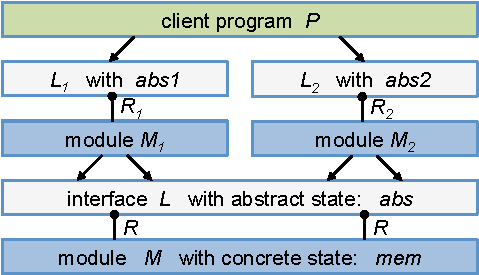
\includegraphics[scale=1]{figs/conflict}
\caption{Client code with conflicting abstract states?}
\hrulefill
\label{fig:conflict}
\end{figure}
%%%%%%%%%%%%%%%%%%%%%%%%%%%%%%%%%%%%%%%%%%%%%%%%%%%%%%%%%%%%%%%%

Deep specification brings out an interesting {\bf new challenge}
shown in Figure~\ref{fig:conflict}: {\em what if a program $P$ attempts to
call primitives defined in two different interfaces $L_1$ and $L_2$,
which may export two conflicting views (i.e., abstract states
\textsf{abs1} and \textsf{abs2}) of the same abstract state \textsf{abs}
(thus also the same concrete memory state \textsf{mem})?}
\ronghui{Concurrency}

Here we assume that modules $M, M_1, M_2$ implement interfaces $L,
L_1, L_2$ via some simulation relations $R, R_1, R_2$ (lines marked
with a dot on one end) respectively. Clearly, calling primitives in
$L_2$ may violate the invariants imposed in $L_1$, and vice versa,
so $L_1$ and $L_2$ are breaking each other's abstraction when we run
$P$. In fact, even without $M_2$ and $L_2$, if we allow $P$ to
directly call primitives in $L$, similar violation of $L_1$ invariants
can also occur.

This means that we must prohibit client programs such as $P$ above,
and each deep specification must state the clear assumptions about its
valid client contexts. Each interface should come with a single
abstract state (\textsf{abs}) used by its primitives; and its client can
only access the same \textsf{abs} throughout its execution. 

This is what {\em abstraction layers} are designed for and why they
are more compositional (with respect to deep specification)
than regular modules! Layers are introduced to limit 
interaction among different modules: only modules with identical
state views (i.e., $R_1, R_2$ and \textsf{abs1},
\textsf{abs2} must be identical) can be composed horizontally.
 
A layer interface seems to be defining a new ``abstract machine''
because it only supports client programs with a particular view of the
memory state. The correctness of a certified layer implementation
allows us to transfer formal reasoning (of client programs) on one
abstract machine (the overlay) to another (the underlay).  

Programming with certified abstraction layers enables a disciplined way of
composing a large number of components in a complex system. Without
using layers, we may have to consider arbitrary module interaction or
dependencies: an invariant held in one function can be easily broken
when it calls a function defined in another module. A layered approach
aims to sort and isolate all components based on a carefully designed
set of abstraction levels so we can reason about one small abstraction
step at a time and eliminate most unwanted interaction and dependencies.



\section{Abstraction Layers for Sequential Kernels}
\label{sec:seq:overview}

\begin{figure}[tb] \centering
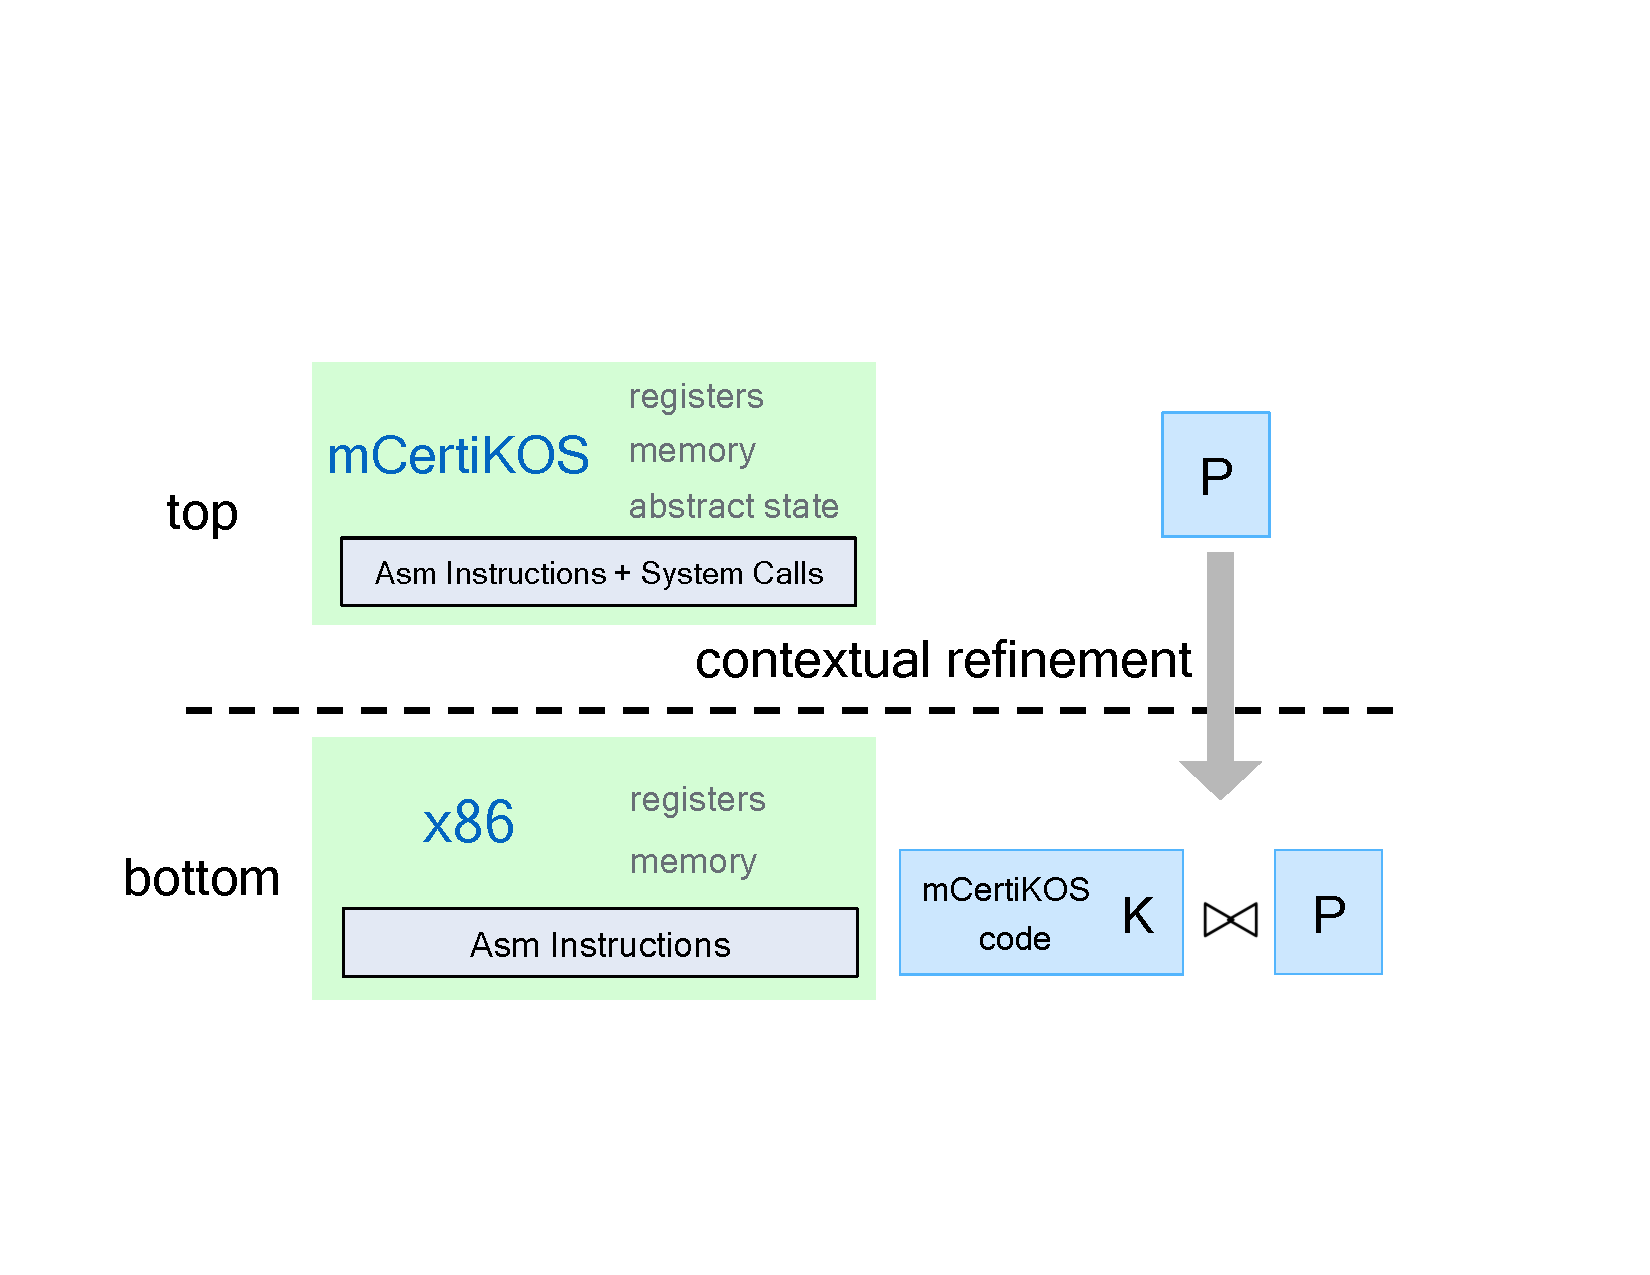
\includegraphics[scale=.5]{figs/mainthm}
\caption{Certified OS kernels: what to prove?}
\hrulefill
%\rule[0in]{\columnwidth}{.15mm}
\label{fig:mainthm}
\end{figure}

Under \CTOS, building a new certified kernel (or experimenting with a new
design) is just a matter of composing a collection of certified
layers, developed in a variant of C (called ClightX) or assembly.
\CTOS{} provides  a powerful Coq library
for supporting {\em horizontal} and {\em vertical} composition of
certified layers, as well as a certified compiler (called
CompCertX) that can compile certified ClightX layers into certified
assembly layers. \CTOS\ can thus enjoy the full programming power of
an ANSI C variant and also the assembly language to certify any
efficient routines required by low-level kernel programming.  The
layer mechanism allows us to certify most kernel components at higher
abstraction levels, even though they all eventually get mapped (or
compiled) down to an assembly machine
 that models important hardware details (\eg, virtual memory support).


In Figure~\ref{fig:mainthm}\ronghui{$\oplus$}, we use x86 to denote an assembly machine
and {$\sem{\rm{}x86}{\cdot}$} for its whole-machine semantics.
Suppose we load such a machine with the \mCTOS\ kernel $K$ (in
assembly) and user-level assembly code $P$; then proving any
global property of such a complete system amounts to reasoning about
the semantic object {$\sem{\rm{}x86}{K\join P}$}.

Reasoning at such a low level is difficult, so we formalize a new
\mCTOS\ machine that extends the x86 machine with the deep
specification of $K$. We use $\sem{\rm\mCTOS}{\cdot}$ to denote its
whole-machine semantics.  The contextual refinement property about the
\mCTOS\ kernel can be stated as $\forall
P,\;\sem{\rm{}x86}{K\join{}P}\Refrel{}\sem{\rm\mCTOS}{P}$.
\noindent{}Hence any global property proved about
$\sem{\rm\mCTOS}{P}$ can be transferred to
$\sem{\rm{}x86}{K\join{}P}$.


%Contextual refinement is also a highly general and
%compositional property. Recent work~\cite{filipovic10,liang13} on
%concurrent objects~\cite{herlihy90} has shown that contextual
%refinement is precisely equivalent to the linearazibility and
%various liveness properties~\cite{Herlihy08book}. 

\begin{figure}[tb] \centering
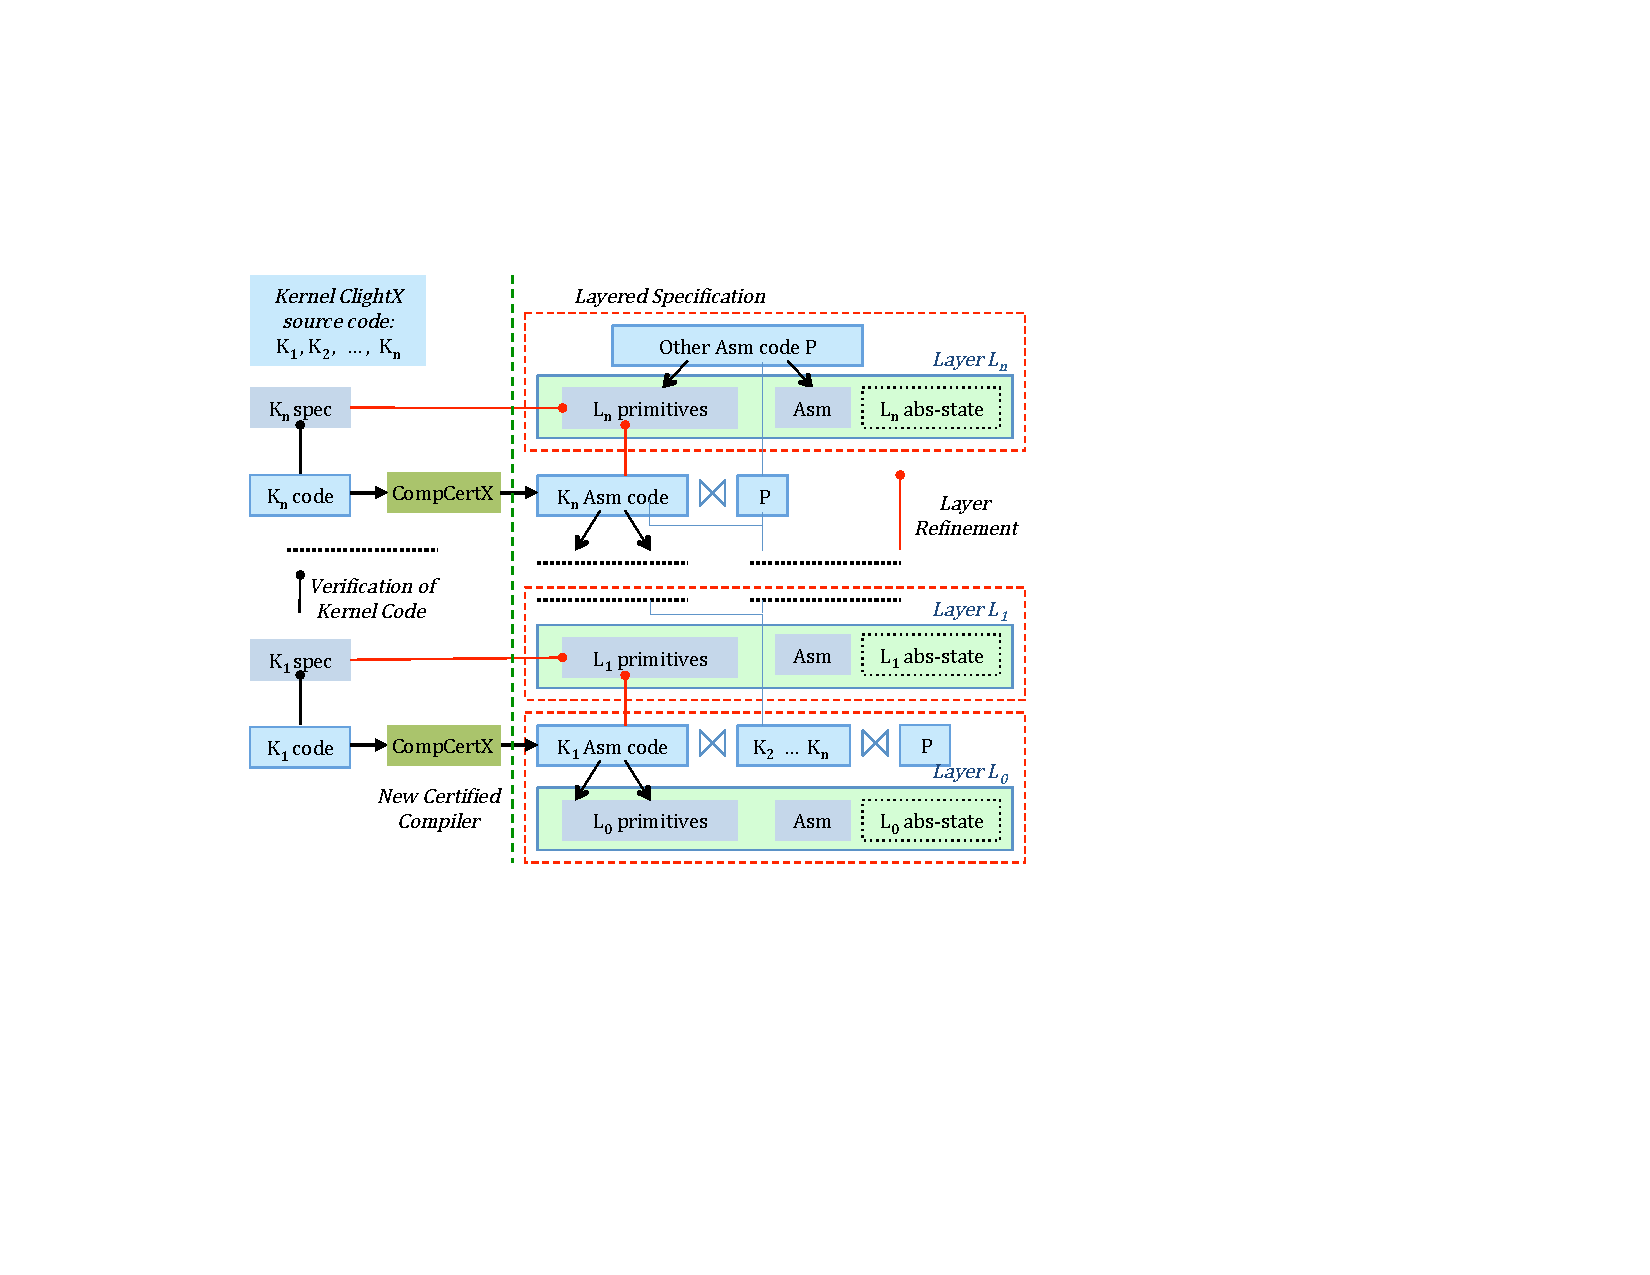
\includegraphics[scale=1]{figs/archA}
\caption{Overview of the \CTOS\ architecture}
\hrulefill
%\rule{\columnwidth}{.15mm}
\label{fig:arch}
\end{figure}

In \CTOS, we also use contextual refinement to support fine-grained
layer decomposition and linking.  In Figure~\ref{fig:arch}, to build a
certified kernel $K$, we decompose it into multiple kernel modules
$K_1,...,K_n$, each sitting at its respective underlay ($L_0$, ...,
$L_{n-1}$). Each such module ($K_i$) implements the primitives in its
overlay (\ie, $L_i$) but it can only call the primitives in its
underlay (\ie, $L_{i-1}$).  Using vertical composition~\cite{dscal15}, from
the contextual refinement $\forall
P,\;\sem{i-1}{K_i\join{}P}\Refrel{}\sem{i}{P}$ for each layer (we use
$\sem{j}{\cdot}$ to denote the semantics of the $L_j$ machine), we can
deduce:
$$\forall P, \sem{0}{K\join{}P} =
\sem{0}{K_1\join{}K_2\cdots\join{}K_n\join{}P} \Refrel
\sem{1}{K_2\cdots\join{}K_n\join{}P} \cdots \Refrel
\sem{n-1}{K_n\join{}P} \Refrel \sem{n}{P}$$
If we instantiate $L_0$
and $L_n$ with the x86 and \mCTOS\ layers, we get precisely the
contextual refinement property of the \mCTOS\ kernel. 

We can also
compose intermediate layers in the same way---this makes it much
easier to modify existing (or add new) certified kernel modules.
For example, once the abstract layer interface
$L_{q2}$
for a sequential thread queue (\cf{}Figure~\ref{fig:queue2}) is introduced,
there is no need to see (or reason about) 
the concrete queue implementations $M_{q1}$
(\cf{}Figure~\ref{fig:queue:c:a})
and the intermediate interfaces $L_{q1}$ (\cf{}Figure~\ref{fig:queue:c:b}). 
Thus, all the code relying on the thread queue module can be verified
at a higher abstraction level using these abstract queue primitives,
which are still {\em realizable} by an efficient assembly implementation
(\ie, Figure~\ref{fig:queue:c:a}).


\ignore{
\begin{figure}[htb]\scriptsize
$$
\begin{array}{l|l}
\begin{array}{l}
\verb+/* memory types */+
\\
\verb+#define MEM_RAM      1+
\\ 
\verb+#define MEM_RESERVED 2+
\\
\verb+#define MEM_ACPI     3+
\\
\verb+#define MEM_NVS      4+ 
\\ 
\verb#struct pmmap {#
\\
\verb#  uintptr_t start;#
\\
\verb#  uintptr_t end;#
\\
\verb#  uint32_t  type;#
\\
\verb#};#                           
\\
\verb#struct pmmap mm[128];#
\end{array}
&
\begin{array}{l}
\verb#Inductive MEMPerm:=#
\\
\verb#| MEM_RESERVED#
\\
\verb#| MEM_USABLE.#
\\
\\
\verb#Inductive pmmap:=#
\\
\verb#| MEMV (start end : Z)#
\\
\verb#       (type : MEMPerm)#
\\
\verb#| MEMUndef.#
\\  
\\
\verb#Definition MM :=#
\\
\verb#       ZMap.t pmmap.#
\end{array}
\\\vspace*{-14pt}
\end{array}
$$ 
\caption{Concrete memory vs. abstract state}
\label{fig:abs-pmmap}
\vspace*{-10pt}
\end{figure}


For example, in $K_1$, we might use an array (in $L_0$ memory) to
implement a physical memory map \verb+mm+ (see Fig.~\ref{fig:abs-pmmap} left,
in C syntax); 
this map describes the physical memory
layout including the size and ``type'' of every memory piece. 
For any code above $L_0$, there is no need to see (or reason
about) such concrete details. Instead, we encapsulate $K_1$
by hiding the array (in $L_0$) and replacing it with a Coq finite map
\verb+MM+ (see Fig.~\ref{fig:abs-pmmap} right) as part of 
the new abstract state in $L_1$. Note, we only need to 
know which memory piece is usable or reserved (\verb+MEMPerm+), 
and we need to add the case \verb+MEMUndef+ to represent the content
of \verb+mm+ before it is initialized. Here \verb+Z+ and \verb+ZMap.t+ 
are Coq's integer and finite map types. The new $L_1$ primitives
can then be specified using the Coq finite map
so $L_1$ code can be verified
at a higher abstraction level, but these primitives
are still {\em realizable} by an efficient assembly implementation
(i.e., $K_1$).}

This last point is important since it means that abstraction
layers in \CTOS\ are introduced strictly to support compositional 
specification and verification. Regardless how many layers we add 
and how we specify the layer primitives, the kernel always has the same 
efficient assembly implementation.

\section{Abstraction Layers for Concurrent Kernels}
\label{sec:overview:concurrent}
To build certified concurrent OS kernels,
we introduce a notion of \emph{certified concurrent abstraction
layer}: a special abstraction layer that 
contains a \emph{shared
global log} to record the shared operations
of the whole system.

\paragraph{Concurrent abstraction layers}
Like a general abstraction layer, each concurrent layer can also
contain thread-private abstract states (refined from the concrete
thread-local in-memory data) and related abstract primitives. However,
the data shared by multiple threads are not represented as abstract
states. Instead, each method call to a shared atomic object is
recorded as an observable event and is appended to the end of a shared
global log. For each shared object, we define a {\em replay} function
that can reconstruct the current shared state from the current global
log. Thus, all shared objects are represented as a single sequence of
logged events with appropriate replay functions.

With concurrency, the machine semantics for each layer (\eg,
$\sem{L}{\cdot}$) is no longer deterministic: for each scheduler
strategy ($\strat{hs}$), it may generate a different global
log. To prove the simulation $\sem{L}{P\oplus{}M} \leq_R \sem{L'}{P}$,
for each scheduler strategy $\strat{hs}$, if running $P\oplus{}M$ on
machine $L$ with $\strat{hs}$ produces a global log $l$, we must find
another scheduler strategy $\stratp{hs}$ such that running $P$ on
machine $L'$ under $\stratp{hs}$ would generate a global log $l'$ that
is related to $l$ via the simulation relation $R$. We will actually
construct a {\em function} that will map $l$ and $\strat{hs}$ into
$l'$ and $\stratp{hs}$. Of course, the simulation relation $R$ over
thread-private states might still be a relation~\cite{dscal15}.

\paragraph{An example of concurrent layers}
%%%%%%%%%%%%%%%%%%%%%%%%%%%%%%
\begin{figure}[t]\centering
\lstinputlisting [language = C, multicols=2] {source_code/ticket_lock_example.c}
\caption{Building certified concurrent layers over a ticket lock}
\label{fig:exp:ticket_lock_example}
\hrulefill
\end{figure}
%%%%%%%%%%%%%%%%%%%%%%%%%%%%%%

The example in Figure~\ref{fig:exp:ticket_lock_example} contains a
client program $P$ which has two threads running on two different
CPUs; each thread makes one call to the atomic primitive $\comm{foo}$
provided by the layer interface $L_{t3}$.

Concurrent object module $M_{t2}$ implements the layer interface $L_{t3}$
but it is built on top of $L_{t2}$.  The $\comm{foo}$ method calls two
atomic primitives $f$ and $g$ in a critical section protected by a
ticket lock~\cite{mcs91}.

The ticket-lock module $M_{t1}$ is built on top of $L_{t1}$ and it
implements $L_{t2}$. Even though the implementation of a ticket lock
contains two shared integer value fields, $\comm{ticket}$ and
$\comm{now}$ (where $\comm{now} \leq \comm{ticket}$ always holds), the
interface $L_{t1}$ only provides the atomic primitives such as
fetch-and-incrementing the $\comm{ticket}$ value, getting the current
$\comm{now}$ value, holding the lock (if the $\comm{now}$ value is
equal to the $\comm{ticket}$ value), and incrementing the $\comm{now}$
value (to release the lock). The current $\comm{ticket}$ and
$\comm{now}$ values can be reconstructed by replaying the global log
(for the $L_{t1}$ machine).  $L_{t1}$ also provides the atomic $\comm{f}$
and $\comm{g}$ events which are later passed on to $L_{t2}$.

\paragraph{Strategy, environment context, and concurrent layer simulation}
Our goal is to show that for each run of $P\oplus{}M_{t2}\oplus{}M_{t1}$
over $L_{t1}$, we can find another run of $P$ over $L_{t3}$ so that the
global logs produced by both runs are related.
To show how we accomplish this, here is
a global log $l_{g1}$ produced from  
a specific run of $P\oplus{}M_{t2}\oplus{}M_{t1}$.
\[
\begin{array}{rl}
l_{g1}:= & \ssame \cons (1.\incticket) \cons
\sdiff \cons (2.\incticket) \cons
\ssame \cons (2.\getnow) \cons
\sdiff \cons (1.\getnow)  \\
& \cons\ssame \cons (1.\holdlock) 
\cons 
\sdiff \cons (2.\getnow) \cons
\sdiff \cons (1.\comm{f}) \cons
\sdiff \cons (2.\getnow) \cons
\sdiff \cons (1.\comm{g}) \\
& \cons
\ssame \cons (1.\incnow) 
\cons \sdiff \cons (2.\getnow) 
\cons
\ssame \cons (2.\holdlock) \cons
\ssame \cons (2.\comm{f}) \cons
\ssame \cons (2.\comm{g}) \\
&\cons
\ssame \cons (2.\incnow) 
\end{array}
\]

Throughout this thesis, we assume that all programs always
start from CPU 1, and before each CPU executes an atomic primitive,
it always yields to the hardware scheduler ($hs$).
We use $\ssame$ to denote a hardware yield to the same CPU,
and $\sdiff$ for a yield to a different CPU; each such symbol
is actually an abbreviation of two consecutive switch events: switch
from CPU $i$ to $hs$ (\ie, $i\switch{}hs$), and then switch from $hs$
to CPU $j$ (\ie, $hs \switch j$).  For example, starting from CPU 1,
$\sdiff$ is an abbreviation of $(1\switch{}hs) \cons (hs\switch 2)$.

We define $\comm{target}(l)$ as the switching destination of the last event in
the log $l$, which can be either 1, 2, or $hs$. The above run,
which produced the global log $l_{g1}$, can be viewed as combining
the following {\em strategies} defined for each CPU and $hs$:
\[
\strat{j} (l)=
\begin{cases}
  j.e & \text{if } (\comm{target}(l) = j) ~~\wedge 
      (l\cons (j.e)) |_{j,hs} \text{ is a prefix of } (l_{g1} |_{j,hs}) \\
\comm{undefined } & \text{otherwise}
\end{cases}
\]
\noindent{}Here, $l |_{j,hs}$ only keeps those events in $l$ that are
related to participants $j$ and $hs$.  For the hardware scheduler's
strategy $\strat{hs}$, this filtering essentially means that
regardless how the CPUs (or threads) are going to play in the interim,
$hs$'s moves will always follow $l_{g1}$.  Because $\strat{hs}$
defines how switching between different CPUs is done, when we define
each CPU's strategy, we filter out other CPUs' events but still keep
those events related to $hs$.

At each step, depending on the destination ($j$) of the current log
($l$), we can query the corresponding strategy $\strat{j}(l)$ to get the
next move for $j$.  For example, if the destination is $hs$, that is,
the log ends with $(\any\switch hs)$, then it is the
hardware scheduler's turn to generate a switch event $(hs\switch \any)$.

These strategies also form a nice decomposition of the global log
$l_{g1}$. To reason about CPU 1 alone, since the machine consists of two CPUs, we only need to construct
its environment context 
\[\oracle_1 := \strat{hs} \bigcup \strat{2}\]

The layer $L_{t2}$ introduces the $\acq$ and $\rel$ primitives
which trigger events $\acq$ and $\rel$ respectively. Running
$P\oplus{}M_{t2}$ over $L_{t2}$ could produce the following  log $l_{g2}$:
\[
\begin{array}{l}
\ssame \cons (1.\acq) \cons
\ssame \cons (1.\comm{f}) \cons
\ssame \cons (1.\comm{g}) \cons
\ssame \cons (1.\rel) 
\cons \sdiff \cons (2.\acq) \cons
\ssame \cons (2.\comm{f}) \cons
\ssame \cons (2.\comm{g}) \cons
\ssame \cons (2.\rel) 
\end{array}
\]

The layer interface $L_{t3}$ introduces the atomic $\comm{foo}$
primitive. Running $P$ over $L_{t3}$ could produce the following shared log
$l_{g3}$:
\[
\ssame \cons (1.\comm{foo})
\cons \sdiff \cons (2.\comm{foo})
\]

To build a simulation, we want to define a function mapping one
layer's log and environment context into those of another layer.  For
example, the function $f_l$, mapping a log over $L_{t1}$ into one over
$L_{t2}$, can be defined as follows: (1) it maps the $\holdlock$ and
$\incnow$ events in $L_{t1}$ to $\acq$ and $\rel$ events in $L_{t2}$; (2) it
drops the $\incticket$ and $\getnow$ events; 
and (3) it merges all the adjacent switch symbols (\eg,
$\ssame \cons \sdiff$ is merged into $\sdiff$).
The following shows that $l_{g2} = f_l (l_{g1})$ is true:
\[
\begin{array}{l}
\hspace*{-1em}\mysout
{\ssame \cons (1.\incticket) \cons
\sdiff \cons (2.\incticket) \cons
\ssame \cons (2.\getnow) \cons
\sdiff \cons (1.\getnow)
}\\
\hspace*{-1em} \cons\ssame \cons (1.\cancel{\holdlock}/\acq) 
\mysout
{\cons 
\sdiff \cons (2.\getnow) \cons
\sdiff 
} 
\ssame \cons (1.\comm{f}) \cons
\mysout
{\sdiff \cons (2.\getnow) \cons
\sdiff
}
\\
\hspace*{-1em}
\cons \ssame \cons (1.\comm{g}) \cons
\ssame \cons (1.\cancel{\incnow}/\rel) 
\cons \sdiff 
\mysout
{\cons (2.\getnow) \cons
\ssame 
}
\cons (2.\cancel{\holdlock}/\acq) 
\\
\hspace*{-1em}
\cons
\ssame \cons (2.\comm{f}) \cons
\ssame \cons (2.\comm{g}) \cons
\ssame \cons (2.\cancel{\incnow}/\rel) 
\end{array}
\]

From $f_l$, we can construct a function $f_{\strat{}}$
that maps each strategy $\strat{j}$ for $L_{t1}$ into one for $L_{t2}$:
\[ 
f_{\strat{}}(\strat{j}) (l'')=
\begin{cases}
j.e' & \text{if } 
\exists l', f_l(l') = l'' \wedge \strat{j}(l') = j.e
\wedge f_l(l'\cons(j.e)) = l'' \cons (j.e') \\
\comm{undefined } & \text{otherwise}
\end{cases}
\]
Here, since many $L_{t1}$ events are dropped in $L_{t2}$,
the $L_{t2}$ strategy $f_{\strat{}}(\strat{j})$ for $j$
has to keep querying $\strat{j}$ until
it also returns an event from $j$ at $L_{t2}$.  For example, let $l'$ be
$\ssame \cons (1.\incticket) \cons \sdiff \cons (2.\incticket) \cons
\ssame \cons (2.\getnow) \cons \sdiff \cons (1.\getnow) \cons \ssame$.
Since $\strat{1} (l') = 1.\holdlock$ and $f_l(l') = \ssame$, we have
$f_{\strat{}}(\strat{1}) (\ssame) =1.\holdlock$.

Finally, from $f_{\strat{}}$ we can construct the function
$f_{\oracle}$ which will map each environment context $\oracle$ for
$L_{t1}$ into one for $L_{t2}$.

\paragraph{Concurrent layer verification and composition}
Reasoning about a concrete strategy is simple, but when we verify
a concurrent module, we cannot assume such a specific environment context.
Instead, to verify
a layer running on CPU~$i$, we have to show that its implementation
meets its specification for all possible environment contexts
$\oracle_i$ that satisfy its ``rely'' invariants.

For example, to show that $\ltyp{L_{t1}[1]}{R}{M_{t1}}{L_{t2}[1]}$, we must
show that the implementation of $\acq$ meets its specification.
This requires us to prove the starvation-freedom of the ticket
lock algorithm. To do so, we can impose the following rely conditions
over $\oracle_1$:
%%%%%%
\begin{itemize} \itemsep 0pt
\item ($\comm{INV}_{hs}$):  $\strat{hs}$ is \emph{fair}, \ie,
  for any CPU $i$, the gap between two $(hs \switch i)$ events
  in the log is less than some constant $m$.
%%%%%%%
\item ($\comm{INV}_{2}$):  $\strat{2}$ will eventually release the
  lock it held, \ie, the number of events generated by CPU~2
  between $(2.\holdlock)$ and $(2.\incnow)$   is less
  than some constant $n$ .
\end{itemize}
%%%%
Therefore, when CPU~1 acquires the lock, the loop iteration (\cf
line 17 in Figure~\ref{fig:exp:ticket_lock_example}) is bound by
$n \times m$, because CPU~2 can generate at most $n$ events before
releasing the lock and $\strat{hs}$ is fair to CPU~2.

Interestingly, we do not need
to prove that CPU~1 \emph{guarantees} to release the lock within $n$
steps in machine $L_{t2}[1]$
when we prove $\ltyp{L_{t1}[1]}{R}{M_{t1}}{L_{t2}[1]}$.  We can restore
this guarantee proof when we prove $\ltyp{L_{t2}[1]}{R}{M_{t2}}{L_{t3}[1]}$
since clearly, each call to $\acq$ in $M_{t2}$ is followed by a call to
$\rel$ within three steps.

Two certified layers are allowed to compose only if each one's guarantee
implies the other's rely. We cannot parallel-compose
$\ltyp{L_{t1}[1]}{R}{M_{t1}}{L_{t2}[1]}$ and 
$\ltyp{L_{t1}[2]}{R}{M_{t1}}{L_{t2}[2]}$;
but we can first get $\ltyp{L_{t1}[1]}{R}{M_{t1}\oplus{}M_{t2}}{L_{t3}[1]}$ and
$\ltyp{L_{t1}[2]}{R}{M_{t1}\oplus{}M_{t2}}{L_{t3}[2]}$, and then compose these to
get $\ltyp{L_{t1}[T]}{R}{M_{t1}\oplus{}M_{t2}}{L_{t3}[T]}$.

\paragraph{Layer architecture for concurrent kernels}

\begin{figure}[t]\centering
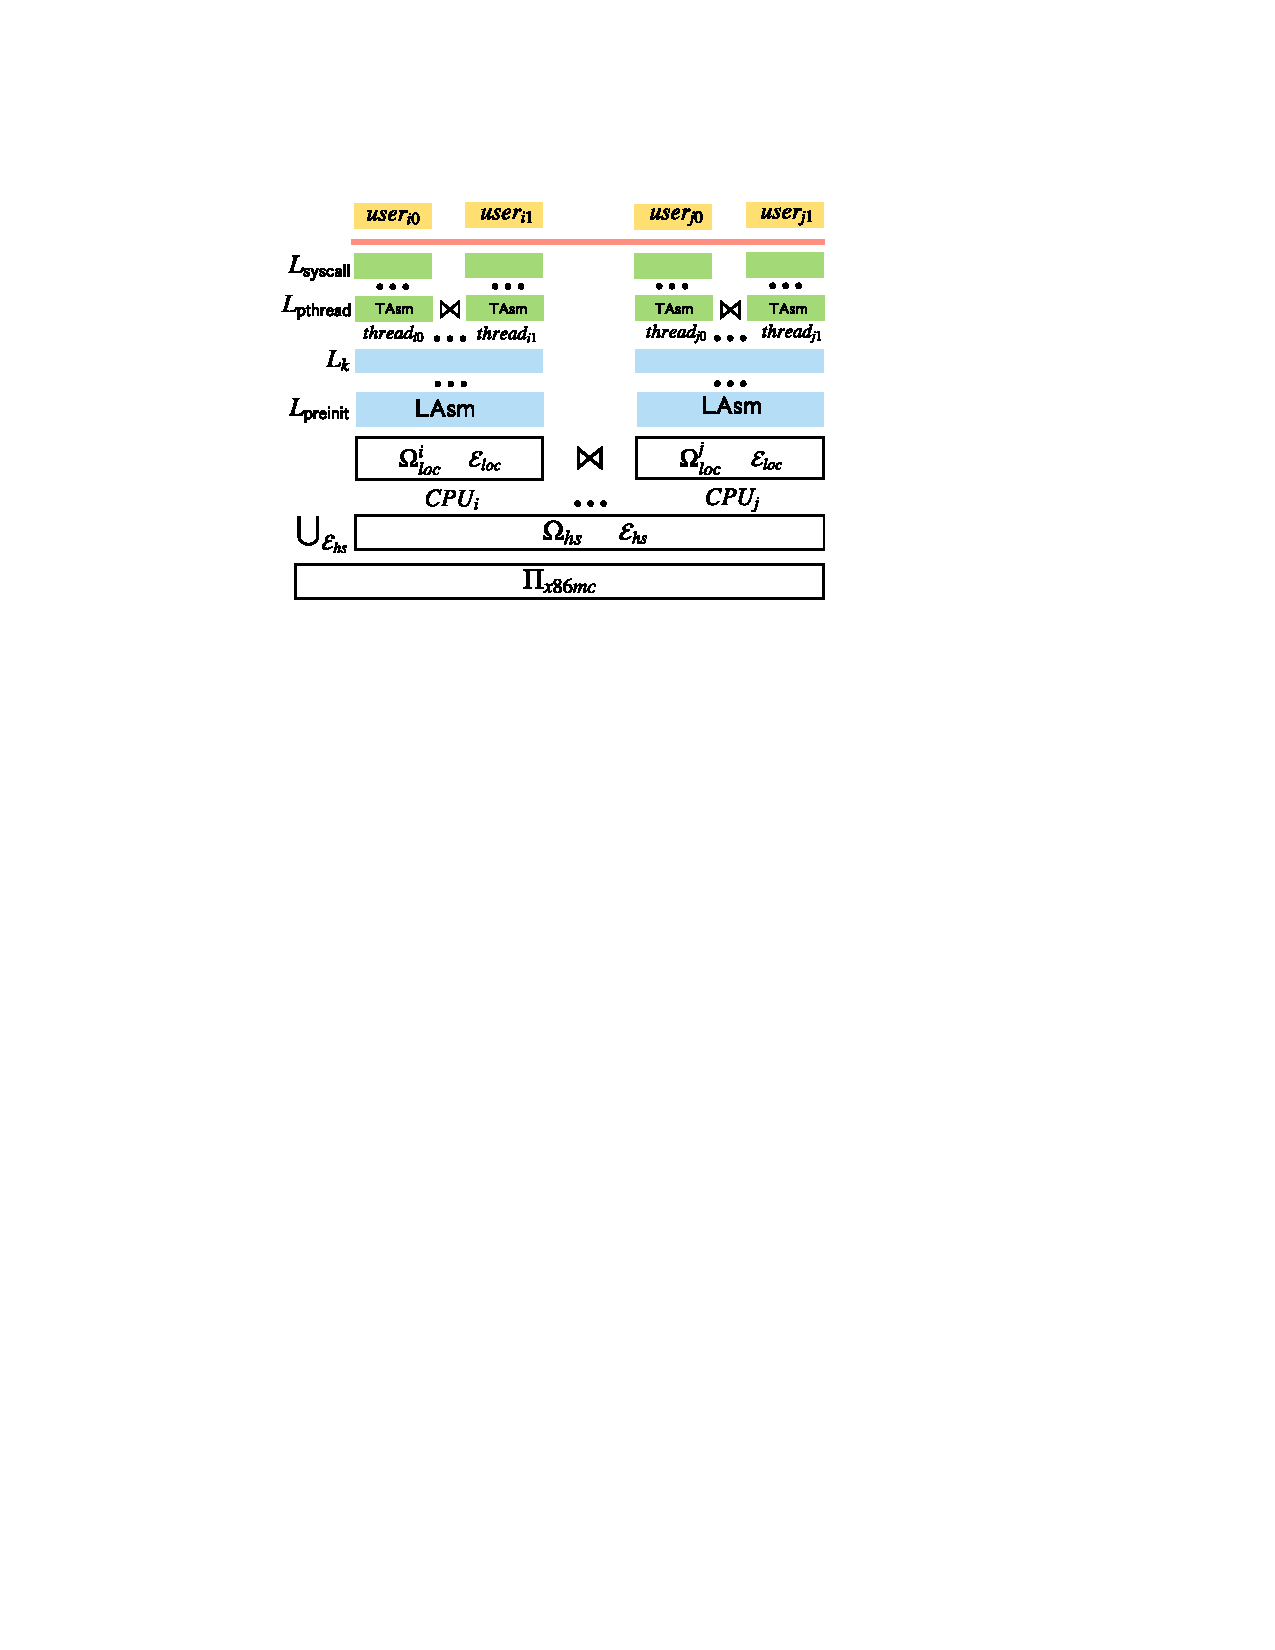
\includegraphics[scale=1]{figs/refine_layer}
\caption{Contextual refinement between concurrent layers.}
\label{fig:spec:refine_layer}
\hrulefill
\end{figure}

With our new compositional concurrent layer interface, as shown in
Figure~\ref{fig:spec:refine_layer}\ronghui{double-check the symbol}, we can freely take a multicore
machine like x86mc and zoom into a specific active core $i$ by
creating a {\em logical} ``single-core'' machine layer for core $i$,
and build
a collection of certified layers
following the same technique shown in Figure~\ref{fig:arch}. 
When we want to introduce kernel- or
user-level threads, we can further zoom into a particular thread
(\eg, $i0$) and create a corresponding logical machine
layer. Eventually, after we have added all the kernel components and
implemented all the system calls, we can combine these per-thread
machines into a single concurrent machine.

\ignore{
\paragraph*{What have we proved?}
Using \CTOS, we have successfully built multiple certified OS
kernels. For each such kernel, we have always constructed its deep
specification and proved its contextual functional correctness
property, so all global properties proved at the specification level can
be transferred down to the lowest assembly machine.

From the functional correctness property, we immediately derive that
all system calls and traps will always run {\em safely} and also
terminate; and there will be no code injection attacks, no buffer
overflows, no null pointer access, no integer overflow, etc. We also
proved that there is no stack overflow or memory exhaustion in the
kernel using recent techniques developed by Carbonneaux~{\em et
  al}~\cite{veristack,ccrb15}.  As we will discuss in
Sec.~\ref{security}, we also proved an isolation property between the
virtual address spaces of user-level processes.  All of these
properties were proved using the abstract specification provided at
the top layer, and then transferred to the lowest assembly machine via
contextual refinement.}